\section{Giới thiệu bài Lab 1}
Mục tiêu của lab 1 như sau:
\begin{itemize}
    \item Hiểu mô hình Agent-Environment
    \item Làm việc với thư viện Gymnasium
    \item Xây dựng Random Agent
    \item Hiểu cách mô hình hóa bài toán thành MDP
    \item Ứng dụng Dynamic Programming trên MDP rời rạc 
\end{itemize}

\section{Phân tích các môi trương Gymnasium}
\subsection{Môi trương CartPole-v1}
\textbf{Môi trường CartPole} mô tả bài toán giữ thăng bằng cho một xe cart có gắn một cột. Mục tiêu của agent là di chuyển chiếc xe theo phương ngang để giữ cho cột luôn thẳng đứng. 
Các thông số của môi trường bao gồm:
\begin{itemize}
    \item Observation space: không gian quan sát bao gồm 4 giá trị liên tục
    \begin{itemize}
        \item \textbf{Cart Position}: Vị trí của xe cart trên mặt phẳng ngang với giới hạn $[-4.8, 4.8]$
        \item \textbf{Cart Velocity}: Vận tốc của xe cart trên mặt phẳng ngang với giới hạn $[-Inf, Inf]$
        \item \textbf{Pole Angle}: Góc nghiêng của cột so với phương thẳng đứng với giới hạn $[-0.418, 0.418]$
        \item \textbf{Pole Angular Velocity}: Vận tốc góc của cột so với phương thẳng đứng với giới hạn $[-Inf, Inf]$
    \end{itemize}
    \item Action space: không gian hành động bao gồm 2 giá trị rời rạc
    \begin{itemize}
        \item \textbf{0}: Di chuyển xe cart sang trái với lực 10 Newton
        \item \textbf{1}: Di chuyển xe cart sang phải với lực 10 Newton
    \end{itemize}
    \item Reward function: hàm thưởng
    \begin{itemize}
        \item \textbf{Thưởng +1}: cho mỗi bước thời gian mà cột luôn thẳng đứng
    \end{itemize}
    \item Trạng thái kết thúc: Cột bị đổ hoặc xe cart ra khỏi giới hạn (trượt quá $4.8$ mét so với vị trí bắt đầu), trò chơi chiến tháng khi đạt được 500 bước mà khôgn làm đổ cột.
\end{itemize}

\subsection{Môi trường MountainCar-v0}
\textbf{Môi trường MountainCar} mô tả bài toán một chiếc xe bị mắc kẹt dưới đáy thung lũng và cần di chuyển để leo lên đỉnh núi. Mục tiêu của agent là di chuyển chiếc xe lên đỉnh núi.
Các thông số của môi trường bao gồm:
\begin{itemize}
    \item Observation space: không gian quan sát bao gồm 2 giá trị liên tục
    \begin{itemize}
        \item \textbf{Cart Position}: Vị trí của xe trên mặt phẳng ngang với giới hạn $[-1.2, 0.6]$
        \item \textbf{Cart Velocity}: Vận tốc của xe trên mặt phẳng ngang với giới hạn $[-0.07, 0.07]$
    \end{itemize}
    \item Action space: không gian hành động bao gồm 3 giá trị rời rạc
    \begin{itemize}
        \item \textbf{0}: Di chuyển xe sang trái
        \item \textbf{1}: Di chuyển xe sang phải
        \item \textbf{2}: Không làm gì
    \end{itemize}
    \item Reward function: hàm thưởng
    \begin{itemize}
        \item \textbf{Thưởng -1}: cho mỗi bước thời gian
    \end{itemize}
    \item Trạng thái kết thúc: Xe đạt đến đỉnh núi hoặc hết thời gian, trò chơi chiến thắng khi đạt được 200 bước mà không bị hỏng
\end{itemize}

\subsection{Trả lời các câu hỏi phân tích}
\begin{itemize}
    \item \textbf{Observation có bao nhiêu chiều?} Đối với CartPole có 4 chiều, đối với MountainCar có 2 chiều
    \item \textbf{State space là liên tục hay rời rạc?} Cả MoutainCar và CartPole đều có state space liên tục
    \item \textbf{Action space là liên tục hay rời rạc?} Cả MoutainCar và CartPole đều có action space rời rạc
    \item \textbf{Reward được tính như thế nào?} Đối với MountainCar, mỗi bước đi có reward -1; còn với CartPole mỗi bước giữ gậy đứng là +1.
    \item \textbf{Khi nào episode kết thúc trong CartPole và MountainCar?} Với MountainCar khi xe đạt đến đỉnh núi hoặc hết thời gian (200 bước); với CartPole khi xe đạt đến giới hạn hoặc hết thời gian (500 bước).
\end{itemize}

\section{Đánh giá Random Agent}
Mội trong những \textbf{Policy} đơn giản nhất trong RL đó chính là chọn ngẫu nhiên hay còn gọi là \textbf{Random Policy} - tức là ta chỉ chọn hành động một cách ngẫu nhiên không quan tâm bất kỳ cái gì.
Trong bài toán \textbf{CartPole}, random agent sẽ chọn hành động 0 hoặc 1 một cách ngẫu nhiên với xác suất 0.5. Khi chạy thử ta có biểu đồ reward - số bước mà agent cân bằng được cây gậy như sau:
\begin{figure}[H]
    \centering
    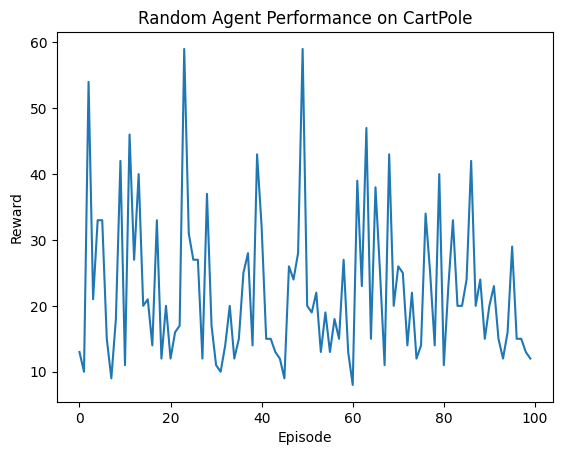
\includegraphics[width=0.8\textwidth]{Images/Lab1/random-cartpole.png}
    \caption{Random Agent - CartPole}
    \label{fig:random_cartpole}
\end{figure}

Với MountainCar, random agent sẽ chọn hành động 0, 1 hoặc 2 một cách ngẫu nhiên với xác suất 0.33. Khi chạy thử ta có biểu đồ reward - số bước mà agent leo lên dốc được như sau:

\begin{figure}[H]
    \centering
    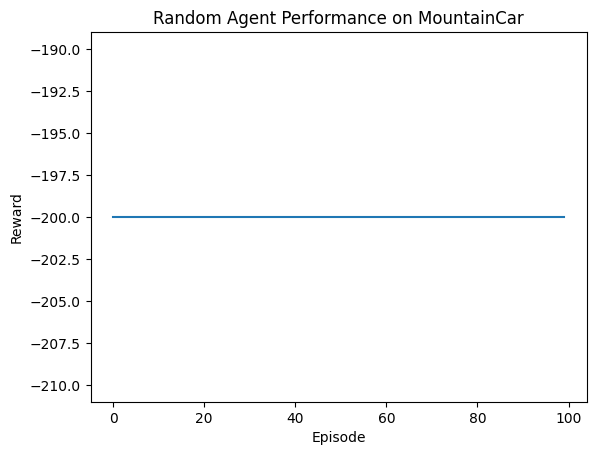
\includegraphics[width=0.8\textwidth]{Images/Lab1/random-mountaincar.png}
    \caption{Random Agent - MountainCar}
    \label{fig:random_mountaincar}
\end{figure}

\textbf{Phân tích kết quả:}
\begin{itemize}
    \item \textbf{Reward trung bình của random agent là bao nhiêu?} Với CartPole là $\approx 22.48$ và với MountainCar là $\approx -200$.
    \item \textbf{Có xu hướng tăng theo thời gian không?} Khi nhìn vào cả hai biểu đồ ta có thể khẳng định là không: đối với CartPole thì dao động đáng kể và không có xu hướng tăng theo thời gian, còn với MountainCar thì hoàn toàn luôn thua - quá 200 bước, chưa bao giờ thắng 1 ván nào cả.
    \item \textbf{Có thể kết luận gì về agent?} Agent không học được gì từ môi trường, vì nó có policy ngẫu nhiên - mọi thứ đều diễn ra ngẫu nhiên và không có sự cải tiến.
    \item \textbf{Vì sao cần một policy học được?} 
    Một policy học được là cần thiết vì nó cho phép Agent biết phân biệt giữa hành động "tốt" và "xấu" thông qua cơ chế phản hồi từ Reward. Khác với Random Policy chỉ chọn hành động mù quáng và không có tính kế thừa, một policy học được có khả năng:
    \begin{itemize}
        \item \textbf{Tối ưu hóa hành vi:} Chuyển từ việc khám phá ngẫu nhiên sang khai thác những kinh nghiệm mang lại phần thưởng cao.
        \item \textbf{Giải quyết các bài toán phức tạp:} Tìm ra những chuỗi hành động logic (như việc lấy đà trong MountainCar) mà các hành động ngẫu nhiên gần như không thể thực hiện được do xác suất quá thấp.
        \item \textbf{Hội tụ:} Đảm bảo hiệu năng của Agent tăng dần theo thời gian và đạt đến trạng thái ổn định tối ưu thay vì dao động không định hướng.
    \end{itemize}
\end{itemize}

\section{Mô hình hóa MDP và Lập trình động cho CartPole}
\subsection{Mô hình hóa MDP}
Môi trường CartPole được mô hình hóa dưới dạng môt tiến trình quyết định Markov (MDP) với các thành phần như sau:
\begin{itemize}
    \item \textbf{Trạng thái ($\mathcal{S}$):} là môt không gian liên tục 4 chiều bao gồm: vị trí xe (\(x\)), vận tốc xe (\(\dot{x}\)), góc nghiêng của cột (\(\theta\)) và vận tốc góc của cột (\(\dot{\theta}\)).
    \item \textbf{Hành động ($\mathcal{A}$):} là tập hữu hạn gồm 2 hành đông rời rạc: \\
    $\mathcal{A} = \{0, 1\}$ (Đẩy trái, đẩy phải).
    \item \textbf{Phần thưởng ($\mathcal{R}$):} một giá trị hằng số $+1$ sau mỗi bước thời gian mà cột chưa bị đổ.
    \item \textbf{Điều kiện kết thúc:} Episode kết thúc khi $|\theta| > 12^{\circ}$ hoặc $|x| > 2.4$ mét hoặc đủ 500 bước.
\end{itemize}
\textbf{Thảo luận:}
\begin{itemize}
    \item \textbf{Tính hữu hạn:} CartPole \textbf{không phải} là một MDP hữu hạn vì không gian quan sát của nó là liên tục. Việc có vô số trạng thái khiến cho tập hợp $S$ có kích thước vô cùng lớn.
    \item \textbf{Khả năng áp dụng DP:} Do số lượng trạng thái là vô hạn, ta không thể áp dụng trực tiếp các thuật toán Lập trình động vốn dựa trên việc tra cứu bảng (Table-lookup). Điều này đặt ra yêu cầu phải \textbf{rời rạc hóa} không gian trạng thái ở các bước tiếp theo.
\end{itemize}

\subsection{Rời rạc hóa không gian trạng thái}
Để có thể áp dụng các thuật toán Lập trình động, ta thực hiện kỹ thuật \textbf{Binning} để chuyển đổi không gian trạng thái liên tục thành không gian rời rạc hữu hạn. 
\textbf{Cấu hình hệ thống:}
Trong bài thực hành này, các biến trạng thái được chia theo cấu hình sau:
\begin{itemize}
    \item Vị trí xe (Cart Position): 4 bins trong khoảng $[-4.8, 4.8]$.
    \item Vận tốc xe (Cart Velocity): 4 bins trong khoảng $[-5.0, 5.0]$.
    \item Góc nghiêng (Pole Angle): 10 bins trong khoảng $[-0.418, 0.418]$.
    \item Vận tốc góc (Pole Angular Velocity): 10 bins trong khoảng $[-5.0, 5.0]$.
\end{itemize}
Như vậy, tổng số trạng thái hữu hạn của mô hình là $4 \times 4 \times 10 \times 10 = 1,600$ trạng thái.

\textbf{Công thức rời rạc hóa:}
Để chuyển đổi một giá trị liên tục $s$ thuộc khoảng $[s_{min}, s_{max}]$ thành một chỉ số rời rạc $i \in \{0, 1, \dots, N-1\}$, ta sử dụng công thức:
\begin{equation}
    i = \text{clip} \left( \left\lfloor \frac{s - s_{min}}{s_{max} - s_{min}} \times N \right\rfloor, 0, N-1 \right)
\end{equation}

Trong mã nguồn Python, cơ chế này được thực hiện hiệu quả bằng thư viện \texttt{numpy} như sau:
\begin{lstlisting}[style=PythonStyle]
def discretize(state):
    # Tinh ti le vi tri cua state trong khoang [MIN, MAX]
    ratio = (state - MIN_VALS) / (MAX_VALS - MIN_VALS)
    # Nhan voi so bins va lam tron xuong de lay chi so
    indices = (ratio * BINS).astype(int)
    # Gioi han chi so trong khoang [0, BINS-1]
    indices = np.clip(indices, 0, np.array(BINS) - 1)
    return tuple(indices)
\end{lstlisting}
Việc sử dụng \texttt{np.clip} là cực kỳ quan trọng để đảm bảo rằng nếu Agent rơi vào các trạng thái ngoại lai (outliers) vượt quá phạm vi quan sát dự kiến, chỉ số trả về vẫn nằm trong giới hạn của ma trận Q-table hoặc ma trận xác suất chuyển trạng thái.

\textbf{Phân tích Trade-off:}
Việc lựa chọn số lượng bins là một bài toán đánh đổi quan trọng:
\begin{itemize}
    \item \textbf{Độ chính xác (Accuracy):} Khi tăng số lượng bins, Agent có khả năng quan sát môi trường mịn hơn, giảm thiểu sai số do việc làm tròn trạng thái, từ đó có thể đạt được Policy tối ưu hơn.
    \item \textbf{Chi phí tính toán và Dữ liệu:} Tuy nhiên, số lượng trạng thái tăng lên sẽ khiến kích thước ma trận xác suất chuyển trạng thái $P(s'|s, a)$ tăng theo bình phương số trạng thái. Điều này không chỉ tốn tài nguyên bộ nhớ mà còn đòi hỏi số lượng mẫu thử (samples) cực lớn để ước lượng chính xác xác suất chuyển giữa các cặp trạng thái, tránh hiện tượng ma trận bị thưa (data sparsity).
\end{itemize}

\subsection{Ước lượng mô hình Model-based}
Sau khi rời rạc hóa, ta cần xây dựng mô hình toán học của môi trường thông qua viêc thu thập mẫu dữ liệu trong môi trường $(s, a, r, s')$.

\textbf{Phương pháp thu thập:} 
Ta sử dụng một policy ngẫu nhiên (random policy) để tương tác với môi trường và thu thập dữ liệu. Trong mỗi bước thời gian, agent sẽ chọn một hành động ngẫu nhiên và ghi lại các thông tin $(s, a, r, s')$.
\textbf{Công thức ước lượng:}
Dựa trên luật số lớn, xác suất chuyển trạng thái $P(s'|s, a)$ và phần thưởng $R(s, a)$ được ước lượng như sau:
\begin{equation}
P(s'|s, a) = \frac{N(s, a, s')}{N(s, a)}
\end{equation}
\begin{equation}
R(s, a) = \frac{R(s, a)}{N(s, a)}
\end{equation}

\textbf{Thảo luận:}
\begin{itemize}
    \item \textbf{Số lượng mẫu cần thiết:} Để mô hình có độ tin cậy cao, mỗi cặp trạng thái - hành động $(s, a)$ cần được thăm thăm đủ số lần. Với không gian 1,600 trạng thái, việc sử dụng 60,000 episodes giúp đảm bảo hầu hết các trạng thái quan trọng gần vùng cân bằng đều được lấy mẫu đầy đủ.
    \item \textbf{Độ chính xác của mô hình:} Mô hình thu được chỉ là một sự xấp xỉ của môi trường thực tế. Độ chính xác phụ thuộc rất lớn vào chiến lược khám phá (exploration). Nếu Random Agent không thể chạm tới một số vùng trạng thái nhất định, ma trận $P$ tại đó sẽ bị rỗng, dẫn đến việc Agent không thể học được hành động tối ưu tại những vùng đó.
\end{itemize}

\subsection{Triển khai thuật toán Value Iteration và Policy Iteration}
Sau ki đã có $P$ và $R$, ta áp dụng thuật toán Value Iteration và Policy Iteration để tìm ra Policy tối ưu.

\textbf{a. Value Iteration:}
Thuật toán này thực hiện vào việc tìm hàm giá trị tối ưu thông qua các bước lặp, dùng phương trình Bellman:
\begin{equation} 
    V_{k+1}(s) = \max_{a \in \mathcal{A}} \left( R(s, a) + \gamma \sum_{s' \in \mathcal{S}} P(s'|s,a) V_k(s') \right) 
\end{equation} 
Trong đó:
\begin{itemize}
    \item $V(s)$ là hàm giá trị của trạng thái $s$.
    \item $R(s, a)$ là phần thưởng khi thực hiện hành động $a$ trong trạng thái $s$.
    \item $\gamma$ là hệ số chiết khấu.
    \item $P(s'|s,a)$ là xác suất chuyển từ trạng thái $s$ sang trạng thái $s'$ khi thực hiện hành động $a$.
\end{itemize}

\textbf{b. Policy Iteration:}
Khác với Value Iteration lặp lại trên hàm giá trị, Policy Iteration chia quá trình học thành việc đánh giá độ tốt của chính sách hiện tại rồi mới thực hiện bước nhảy vọt để cải thiện nó. Điều này giúp Policy Iteration thường hội tụ sau rất ít vòng lặp lớn, mặc dù chi phí tính toán trong mỗi vòng lặp là cao hơn.

\subsection{Đánh giá kết quả và So sánh}
Sau khi tối ưu hóa các tham số rời rạc hóa (BINS = [1, 1, 24, 24]) và bổ sung bộ đếm thời gian thực thi, kết quả thực nghiệm được tổng hợp như sau:

\begin{table}[H]
\centering
\begin{tabular}{lccc}
\toprule
\textbf{Phương pháp} & \textbf{Số vòng lặp (Train)} & \textbf{Thời gian (s)} & \textbf{Reward trung bình} \\
\midrule
Random Agent & 0 & 0.0449 & 22.02 \\
Value Iteration (VI) & 1,376 & 9.8325 & 42.53 \\
Policy Iteration (PI) & 20* & 64.2567 & 12.22 \\
\bottomrule
\end{tabular}
\caption{So sánh hiệu năng các thuật toán trên môi trường CartPole-v1}
\label{tab:ketqua_final}
\end{table}
\textit{* Thuật toán dừng cưỡng bức ở 20 vòng lặp để tránh vòng lặp vô hạn.}
\textbf{Phân tích kết quả:}
\begin{itemize}
    \item \textbf{Về tốc độ hội tụ:} 
    Policy Iteration chạm giới hạn 20 vòng lặp mà chưa hội tụ hoàn toàn, trong khi Value Iteration cần 1,376 vòng lặp để đạt tiêu chuẩn hội tụ. Xét về thời gian thực thi thực tế, \textbf{Value Iteration nhanh hơn (9.83s)} so với Policy Iteration (64.26s). Sự chênh lệch lớn này là do mỗi vòng lặp của PI đều thực hiện bước đánh giá chính sách (Policy Evaluation) lặp đi lặp lại trên toàn bộ không gian trạng thái, dẫn đến khối lượng tính toán cực lớn.
    
    \item \textbf{Về hiệu năng điều khiển (Average Reward):}
    \begin{itemize}
        \item \textbf{Random Agent:} Đạt mức trung bình 22.02 điểm, đóng vai trò là mức cơ sở (baseline) để so sánh.
        \item \textbf{Value Iteration:} Đạt kết quả tốt nhất trong thí nghiệm này với \textbf{42.53 điểm} (cao gấp gần 2 lần so với Random Agent). Điều này cho thấy thuật toán đã tìm được một chính sách điều khiển có ý nghĩa từ dữ liệu mẫu.
        \item \textbf{Policy Iteration:} Chỉ đạt 12.22 điểm, thấp hơn cả Random Agent. Kết quả kém này là hệ quả của việc thuật toán không thể hội tụ trong 20 vòng lặp, khiến chính sách thu được vẫn còn nhiễu và chưa tối ưu.
    \end{itemize}
\end{itemize}
\textbf{Kết luận:} 
Thí nghiệm cho thấy mặc dù các thuật toán Lập trình động có tiềm năng tối ưu hóa chính sách, hiệu quả của chúng phụ thuộc chặt chẽ vào sự hội tụ và chất lượng mô hình MDP ước lượng. Trong trường hợp này, Value Iteration tỏ ra ổn định hơn. Sự thất bại của Policy Iteration trong việc hội tụ cũng nhấn mạnh thách thức khi áp dụng DP vào không gian trạng thái liên tục đã được rời rạc hóa, nơi các vòng lặp vô hạn hoặc sự dao động chính sách có thể xảy ra.
